% Compile with pdfLaTeX or XeLaTeX (Overleaf default pdfLaTeX works out-of-the-box)
% Standard IEEE Conference Template: 10pt body, 12pt single-spaced leading, two-column
\documentclass[10pt,conference]{IEEEtran}
\IEEEoverridecommandlockouts

\usepackage{cite}
\usepackage{amsmath,amssymb,amsfonts,amsthm}
\usepackage{algorithm}
\usepackage{algorithmic}
\usepackage{graphicx}
\usepackage{textcomp}
\usepackage{xcolor}
\usepackage{booktabs}
\usepackage{multirow}
\usepackage{url}
\usepackage{microtype}

\newtheorem{proposition}{Proposition}

\begin{document}

\title{Heterogeneity-Aware Edge-Cloud Speculative Decoding over Wide-Area Networks: Analytical Modeling, Variable-Budget Static Graph Verification, and Empirical Analysis}

\author{%
  \IEEEauthorblockN{Course Research Paper --- Distributed Systems \& Edge-Cloud Collaboration}
  \IEEEauthorblockA{\textit{Cross-Platform Heterogeneous Testbed: RTX 4080 SUPER (32\,GB) $\times$ RTX 5060 Ti (8\,GB) $\times$ Apple M4 (16\,GB)}\\
  Code \& Artifacts: \texttt{https://github.com/davidmartin2077/specedge-reproduction}}
}

\maketitle

\begin{abstract}
Edge-assisted speculative decoding, exemplified by SpecEdge, alleviates the memory-bandwidth bottleneck of autoregressive Large Language Model (LLM) serving by offloading lightweight draft tree generation to edge devices while retaining batched target-model verification on a central server. However, existing evaluations rely on an idealized deployment model: homogeneous Linux nodes with NVIDIA CUDA accelerators connected over sub-millisecond 10\,GbE local-area networks. In practical laboratory and consumer device-cloud clusters---where discrete desktop GPUs and Apple Silicon laptops collaborate over Wide-Area Networks (WANs) such as Tailscale---edge nodes exhibit severe three-dimensional heterogeneity across execution backends (CUDA Graph vs.\ eager PyTorch MPS), memory capacity (8\,GB discrete VRAM vs.\ 16\,GB unified memory), and network round-trip latency (500--1500\,ms).

Through 18 controlled-variable experiments on a real cross-platform three-node cluster serving \texttt{Qwen3-14B} on \texttt{SpecBench}, we uncover a counter-intuitive throughput inversion in which a faster GPU edge trails a slower laptop edge under uniform speculation policies. To explain and resolve this phenomenon, we make three research contributions: (1)~an analytical Time-Per-Output-Token (TPOT) model and dimensionless bottleneck ratio $\rho = (T_{\mathrm{net}} + T_{\mathrm{verify}}) / T_{\mathrm{draft}}$ that predicts divergent optimal tree depths for network-bound ($\rho \gg 1$) versus compute-sensitive ($\rho \approx 1$) edges ($R^2 = 0.992$), along with a fixed dispatch-overhead amortization effect on Apple Silicon; (2)~a non-intrusive Apple MPS compatibility layer and a lightweight \emph{Variable-Budget Static CUDA Graph Zero-Padding} server mechanism that concurrently serves heterogeneous tree budgets from a single captured graph with mathematically equivalent verification and only $+2.0$\,ms overhead; and (3)~a heterogeneity-aware edge configuration policy that boosts bottleneck-node throughput by \textbf{+57.7\%}, cuts server RPCs by \textbf{28.9\%}, reduces laptop local draft compute by \textbf{64.0\%}, raises cluster aggregate throughput by \textbf{+9.7\%}, and lowers inter-edge throughput imbalance from $2.20\times$ to $1.23\times$.
\end{abstract}

\begin{IEEEkeywords}
Edge-cloud collaborative inference, speculative decoding, heterogeneous edge computing, CUDA Graphs, Apple Silicon MPS, wide-area networks.
\end{IEEEkeywords}

\section{Introduction}

Serving Large Language Models (LLMs) interactively remains fundamentally constrained by GPU memory bandwidth during autoregressive token generation~\cite{leviathan2023spec}. Because each decoded token requires streaming billions of target-model parameters from High Bandwidth Memory (HBM) with low arithmetic intensity, expensive high-VRAM servers frequently operate far below their peak compute throughput. Tree-structured speculative decoding~\cite{svirschevski2024specexec} mitigates this inefficiency by employing a small draft model to propose a branching tree of candidate continuations that the target model verifies in a single parallel forward pass, preserving the exact target output distribution.

Building on this principle, SpecEdge~\cite{park2025specedge} introduced an edge-assisted serving architecture in which edge devices execute draft tree construction locally and transmit only compact token IDs and tree attention masks over gRPC to a shared cloud or server verifier. By decoupling drafting from verification, the central server dedicates its full VRAM capacity to the target LLM and static CUDA Graphs.

Despite its strong performance in controlled datacenter setups, deploying SpecEdge in realistic academic and consumer device-cloud environments exposes a stark mismatch with the original paper's assumptions:
\begin{enumerate}
  \item \textbf{Backend and Memory Asymmetry:} Real edge pools routinely mix discrete NVIDIA GPUs (supporting low-overhead CUDA Graphs but constrained to 8\,GB consumer VRAM) with thin-and-light Apple Silicon laptops (offering 16\,GB unified memory but running PyTorch MPS in eager kernel-dispatch mode without CUDA Graph capture).
  \item \textbf{Wide-Area Network Heterogeneity:} Personal and cross-campus devices commonly interconnect via overlay VPNs (e.g., Tailscale) across commodity WAN links, introducing asymmetric Round-Trip Times (RTTs) of 500--1500\,ms---three orders of magnitude higher than 10\,GbE LANs ($<1$\,ms).
  \item \textbf{Uniform Budget Lock-In:} SpecEdge's server verification engine allocates fixed-shape static CUDA Graph tensors sized to a single global \texttt{max\_budget}, forcing every concurrent edge device to share identical tree budgets regardless of local compute speed or link latency.
\end{enumerate}

During initial three-node integration, we observed a striking anomaly: an \texttt{RTX 5060 Ti} edge running \texttt{Qwen3-1.7B} with CUDA Graphs achieved \emph{lower} end-to-end decode throughput (2.78\,tok/s) than an \texttt{Apple M4} laptop running the smaller \texttt{Qwen3-0.6B} under eager MPS dispatch (3.31\,tok/s). This throughput inversion raises three core research questions:
\begin{itemize}
  \item \emph{RQ1:} How do execution backend overhead, draft model scale, and WAN RTT interact quantitatively to govern per-token latency in heterogeneous edge-cloud speculative decoding?
  \item \emph{RQ2:} Do uniform speculation budgets and default Proactive Drafting heuristics remain optimal across network-bound and compute-sensitive edge nodes?
  \item \emph{RQ3:} Can a single static-graph target server concurrently accommodate per-client heterogeneous tree budgets without graph recompilation, memory inflation, or accuracy loss?
\end{itemize}

To answer these questions, we conduct an end-to-end modeling, system design, and controlled-variable empirical study across three physical machines (WSL2 RTX 4080 SUPER server, Windows RTX 5060 Ti edge, and macOS Apple M4 edge). Our main contributions are summarized as follows:
\begin{itemize}
  \item \textbf{Analytical Regime Modeling:} We formulate a closed-form heterogeneous WAN TPOT model and introduce a dimensionless bottleneck ratio $\rho$ that cleanly separates network-bound ($\rho \gg 1$) and compute-sensitive ($\rho \approx 1$) regimes, predicting opposite optimal tree depths and explaining an empirical dispatch-overhead amortization effect on Apple MPS.
  \item \textbf{Cross-Platform MPS Compatibility:} We engineer a zero-overhead device-dispatch compatibility layer enabling SpecEdge on Apple Silicon MPS, resolving a latent non-graph \texttt{KVCache.seq\_indices} slicing bug and Windows Python 3.14 gRPC teardown hangs.
  \item \textbf{Variable-Budget Static CUDA Graph Zero-Padding:} We design and formally justify a single-graph zero-padding verifier with dummy-slot KV isolation and masked KV reordering, allowing concurrent heterogeneous budgets ($B{=}64$ and $B{=}16$) at only $+2.0$\,ms verification overhead.
  \item \textbf{Controlled-Variable Empirical Validation:} Across four progressive experimental suites (18 configurations on \texttt{SpecBench}), we validate our analytical predictions ($R^2{=}0.992$) and demonstrate $+57.7\%$ bottleneck speedup, $-64.0\%$ laptop draft compute reduction, and $+9.7\%$ cluster aggregate throughput gain under real three-node concurrency.
\end{itemize}

\section{Related Work}

\subsection{Speculative and Tree-Based LLM Decoding}

Lossless speculative decoding~\cite{leviathan2023spec,chen2023accelerating} accelerates autoregressive generation by pairing a fast draft model with exact rejection sampling against a larger target LLM. Early chain-based schemes accept at most one linear path per verification step, leaving GPU parallelism underutilized when per-token acceptance probabilities are moderate. Subsequent works generalize speculation into candidate trees verified via customized tree-attention masks: Medusa~\cite{cai2024medusa} attaches multiple decoding heads to the target backbone, EAGLE~\cite{li2024eagle} extrapolates hidden features across tree levels, and SpecExec~\cite{svirschevski2024specexec} builds massively parallel candidate trees using a standalone small draft model tailored to consumer hardware. While these methods optimize single-machine arithmetic intensity, they do not model wide-area network latency or cross-platform backend heterogeneity between draft and target nodes.

\subsection{Edge-Cloud Collaborative LLM Inference}

Device-cloud collaborative serving partitions LLM workloads across resource-constrained edges and high-capacity servers to reduce cloud cost, preserve local responsiveness, and utilize idle edge compute~\cite{kang2017neurosurgeon,hao2024hybrid}. Split-layer inference transmits high-dimensional intermediate activations across the network, incurring severe bandwidth overhead over WAN links. SpecEdge~\cite{park2025specedge} overcomes activation-transfer bottlenecks by shifting to token-level collaboration: edge clients run a compact draft model and transmit only integer token trees and compact metadata over gRPC, while incorporating Proactive Drafting to overlap subsequent drafting with server waiting. However, SpecEdge evaluates homogeneous CUDA edge clients over 10\,GbE LANs and enforces a single uniform tree budget across all clients. Our work extends edge-assisted speculative decoding into realistic heterogeneous WAN clusters, revealing when uniform policies fail and demonstrating how to adapt tree budgets per device.

\subsection{Static Graph Serving and Accelerator Heterogeneity}

Minimizing host-side kernel launch overhead is critical for small-batch LLM decoding~\cite{kwon2023vllm,agrawal2024sarathi}. NVIDIA CUDA Graphs record an entire forward pass into a replayable GPU command graph, eliminating per-operator CPU dispatch latency, but require fixed input tensor shapes and memory addresses. Conversely, PyTorch's Metal Performance Shaders (MPS) backend on Apple Silicon lacks an equivalent general CUDA Graph capture API, executing transformer layers eagerly with substantial per-layer Python/Metal dispatch overhead. Prior multi-shape CUDA Graph systems either capture multiple graph buckets (multiplying static activation memory) or fall back to eager execution on shape mismatches. Our Variable-Budget Zero-Padding mechanism avoids multi-graph VRAM overhead on a 32\,GB server serving a 14B FP16 target model by padding smaller trees into a single captured graph while isolating dummy KV writes.

\section{Analytical Modeling of Heterogeneous WAN Speculative Decoding}

\subsection{Cycle-Level TPOT Formulation}

Consider an edge device $h \in \{\text{5060Ti}, \text{M4}\}$ executing a draft model of scale $m \in \{0.6\text{B}, 1.7\text{B}\}$ with speculation tree hyperparameters $(d, B)$---where $d$ denotes the maximum tree depth (\texttt{max\_beam\_len}) and $B$ denotes the candidate node budget (\texttt{max\_budget})---and Proactive Drafting mode $p \in \{\texttt{disabled}, \texttt{excluded}, \texttt{included}\}$. Each verification cycle produces $\tau$ accepted tokens from the target model. We model the steady-state Time-Per-Output-Token (TPOT) as:
\begin{equation}
  \mathrm{TPOT}(h,m,d,B,p) = \frac{T_{\mathrm{draft}} + T_{\mathrm{verify}} + T_{\mathrm{net}} + T_{\mathrm{post}} - T_{\mathrm{overlap}}}{\mathbb{E}[\tau(m, d, B, p)]},
  \label{eq:tpot}
\end{equation}
where each component captures a distinct hardware or network physical mechanism:
\begin{itemize}
  \item \textbf{Edge Draft Latency ($T_{\mathrm{draft}}$):} Tree construction proceeds depth-by-depth across $d$ draft model forward steps, scaling linearly with depth:
  \begin{equation*}
    T_{\mathrm{draft}}(h, m, d) \approx c_0(h, m) + \alpha(h, m)\cdot d,
  \end{equation*}
  where $c_0(h, m)$ aggregates fixed per-cycle dispatch overhead and $\alpha(h, m)$ is the marginal per-layer execution slope. On CUDA Graph edges, $\alpha$ is small ($\sim 22$\,ms/layer), whereas on eager MPS edges, per-operator host launch overhead inflates $\alpha$ by nearly $6\times$ ($\sim 130$\,ms/layer).
  \item \textbf{Server Verification Latency ($T_{\mathrm{verify}}$):} Under a static CUDA Graph on the 14B target server, verifying $B+1 \le 65$ candidate nodes remains bandwidth-bound on model weights and nearly invariant to $B$ ($75$--$85$\,ms).
  \item \textbf{Network and Host Overheads ($T_{\mathrm{net}}, T_{\mathrm{post}}$):} $T_{\mathrm{net}}(h)$ captures WAN serialization, Tailscale routing RTT, and queueing delay, while $T_{\mathrm{post}}(h)$ measures client-side tree pruning and tensor post-processing.
  \item \textbf{Proactive Overlap ($T_{\mathrm{overlap}}$):} When Proactive Drafting is active, the edge speculatively drafts the next cycle during the server waiting window $T_{\mathrm{wait}} = T_{\mathrm{net}}(h) + T_{\mathrm{verify}}(B)$, hiding up to $T_{\mathrm{overlap}} \le \min(T_{\mathrm{draft}}^{\mathrm{pro}}, T_{\mathrm{wait}})$ when the optimistic continuation is accepted.
  \item \textbf{Mean Accepted Tokens ($\mathbb{E}[\tau]$):} Because conditional acceptance probability decays geometrically along deeper branches, $\mathbb{E}[\tau]$ grows monotonically yet sublinearly with depth $d$, well approximated by a power law $\mathbb{E}[\tau(d)] \approx \kappa d^{\gamma}$ ($0 < \gamma < 1$).
\end{itemize}

\subsection{Dimensionless Bottleneck Ratio $\rho$ and Regime Bifurcation}

To classify heterogeneous edges on a unified scale, we define the dimensionless \emph{Network-to-Draft Bottleneck Ratio}:
\begin{equation}
  \rho(h, m) = \frac{T_{\mathrm{net}}(h) + T_{\mathrm{verify}}}{T_{\mathrm{draft}}(h, m)} = \frac{T_{\mathrm{wait}}}{T_{\mathrm{draft}}(h, m)}.
  \label{eq:rho}
\end{equation}
Neglecting small $T_{\mathrm{post}}$ variation with $d$ and differentiating $\ln \mathrm{TPOT}$ in~(\ref{eq:tpot}) with respect to tree depth $d$, deepening the speculation tree reduces TPOT ($\partial \mathrm{TPOT}/\partial d < 0$) if and only if the relative acceptance gain exceeds the relative cycle-time increase:
\begin{equation}
  \frac{\mathrm{d}\ln \mathbb{E}[\tau]}{\mathrm{d}d} > \frac{\alpha(h, m)}{T_{\mathrm{draft}}(d) + T_{\mathrm{wait}}}.
  \label{eq:opt_cond}
\end{equation}
Substituting $\mathbb{E}[\tau(d)] \approx \kappa d^{\gamma}$ yields $\frac{\gamma}{d} > \frac{\alpha}{c_0 + \alpha d + T_{\mathrm{wait}}}$, from which we directly obtain our central analytical result.

\begin{proposition}[Divergent Optimal Tree Depth]
\label{prop:bifurcation}
Under linear draft scaling and sublinear acceptance growth ($0 < \gamma < 1$), the TPOT-minimizing tree depth satisfies
\begin{equation*}
  d^{*} \approx \frac{\gamma}{1 - \gamma}\cdot\frac{c_0(h, m) + T_{\mathrm{wait}}}{\alpha(h, m)}.
\end{equation*}
Consequently, heterogeneous edges split into two opposing regimes:
(i)~\textbf{Network-Bound Regime ($\rho \gg 1$, small $\alpha$):} $T_{\mathrm{wait}} / \alpha$ is large, pushing $d^{*}$ beyond typical budget caps; aggressive deep trees ($d{=}8, B{=}64$) strictly reduce TPOT by amortizing high WAN RTT across more accepted tokens.
(ii)~\textbf{Compute-Sensitive Regime ($\rho \approx 1$, large $\alpha$):} $T_{\mathrm{wait}} / \alpha$ is small, yielding an interior shallow optimum ($d^{*} \approx 2$); deeper trees inflate $T_{\mathrm{draft}}$ faster than $\mathbb{E}[\tau]$ grows, causing TPOT to rebound.
\end{proposition}

\subsection{Dispatch-Overhead Amortization on Eager Accelerators}

Equation~(\ref{eq:tpot}) also predicts a counter-intuitive model-scaling effect on eager backends such as Apple Silicon MPS. Suppose upgrading the draft model from $m_1$ (0.6B) to $m_2$ (1.7B) increases computation per layer modestly while leaving a large fixed Python/Metal dispatch floor $c_0$ mostly unchanged. Then $\mathrm{TPOT}(m_2) < \mathrm{TPOT}(m_1)$ holds whenever
\begin{equation}
  \frac{\mathbb{E}[\tau(m_2)]}{\mathbb{E}[\tau(m_1)]} > 1 + \frac{\Delta T_{\mathrm{draft}}}{T_{\mathrm{draft}}(m_1) + T_{\mathrm{wait}} + T_{\mathrm{post}}}.
  \label{eq:amort}
\end{equation}
Because the denominator includes both the large eager dispatch floor and $T_{\mathrm{wait}}$, a modest acceptance improvement ($+8.3\%$ in our measurements) outweighs the incremental compute cost of a $2.8\times$ larger draft model, yielding a net throughput gain.

\section{System Architecture and Core Design}

Fig.~\ref{fig:arch} illustrates our cross-platform three-node collaborative serving architecture and per-cycle WAN execution pipeline. Below we detail the two system components engineered to realize heterogeneity-aware serving on top of SpecEdge.

\begin{figure*}[t]
  \centering
  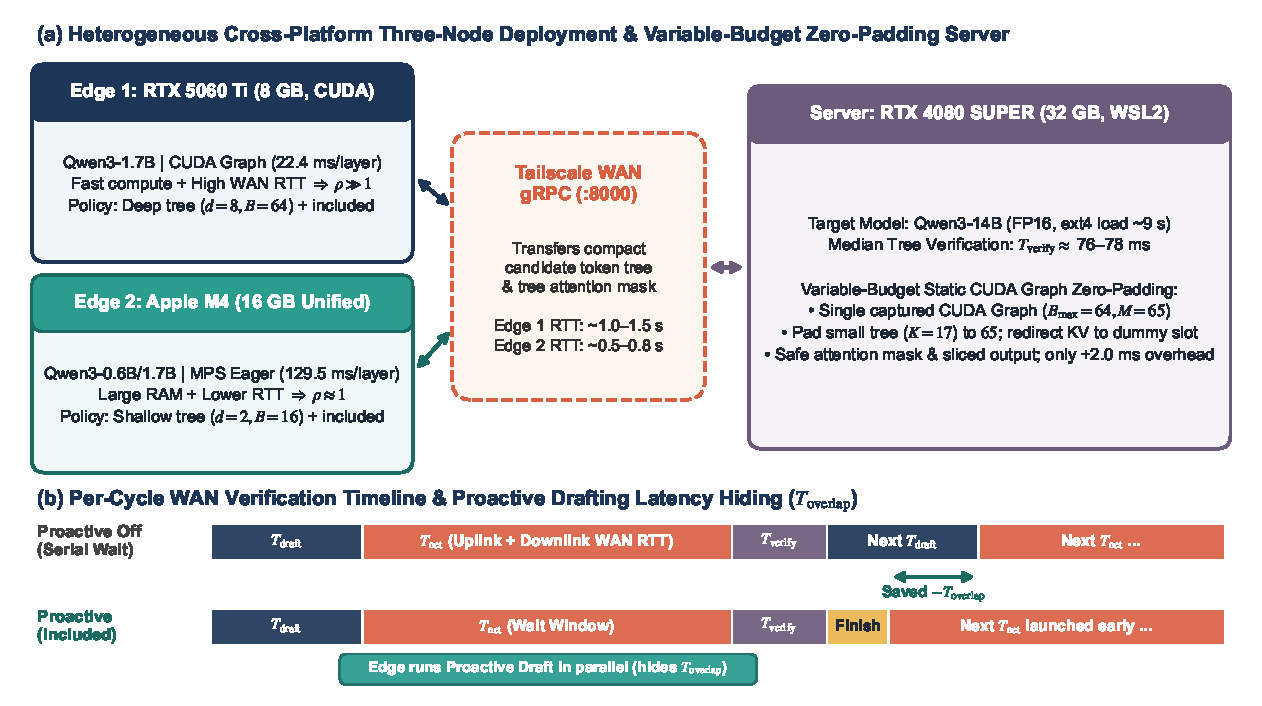
\includegraphics[width=0.96\textwidth]{figures_en/fig1_architecture_timeline.pdf}
  \caption{Cross-platform heterogeneous SpecEdge architecture and WAN pipeline. (a)~A single RTX 4080 SUPER server running \texttt{Qwen3-14B} concurrently serves a network-bound CUDA edge (RTX 5060 Ti, $d{=}8, B{=}64$) and a compute-sensitive MPS edge (Apple M4, $d{=}2, B{=}16$) using one static CUDA Graph via Variable-Budget Zero-Padding. (b)~Under high WAN RTT, Proactive Drafting (\texttt{included}) overlaps next-cycle draft construction ($T_{\mathrm{overlap}}$) inside the network waiting window.}
  \label{fig:arch}
\end{figure*}

\subsection{Non-Intrusive Cross-Platform Apple MPS Compatibility Layer}

Stock SpecEdge hardcodes NVIDIA CUDA primitives throughout its draft engine and profiling utilities, preventing execution on Apple Silicon macOS clients. We design a zero-overhead compatibility layer that preserves identical CUDA execution paths while unlocking native PyTorch MPS support:
\begin{itemize}
  \item \textbf{Device-Aware Graph Fallback and KV-Cache Slicing Fix (\texttt{src/specedge/engine/graph.py}):} During initialization of \texttt{GraphEngine} and \texttt{BatchGraphEngine}, we inspect \texttt{self.\_device.type}. Non-CUDA backends (\texttt{mps}, \texttt{cpu}) automatically bypass \texttt{torch.cuda.CUDAGraph} capture and execute eagerly. While validating variable-width candidate trees on MPS, we uncovered and fixed a latent bug in upstream SpecEdge's non-graph branch: \texttt{forward()} passed the full \texttt{self.\_past\_key\_values.seq\_indices} buffer without slicing \texttt{[:num\_beams]}, causing shape mismatch exceptions (\texttt{[32, 8, 128]} vs.\ \texttt{[1, 8, 128]}) whenever the active beam count was smaller than the pre-allocated budget. Slicing \texttt{seq\_indices[:num\_beams]} resolves this defect across all non-graph backends.
  \item \textbf{Cross-Backend Synchronization and Clean Teardown (\texttt{src/util.py}, \texttt{src/script/client.py}):} We generalize the \texttt{Timing} context manager to dispatch \texttt{torch.mps.synchronize()} on Apple Silicon and automatically fall back from CUDA \texttt{event} timers to wall-clock \texttt{sync} timers on non-CUDA devices. On Windows Python 3.14, we additionally flush logging handlers and explicitly terminate the process upon completing all scheduled requests, eliminating an asynchronous \texttt{grpc.aio} shutdown hang.
\end{itemize}

\subsection{Variable-Budget Static CUDA Graph Zero-Padding Verification}

A key architectural barrier in stock SpecEdge (\texttt{src/strategy/server\_verify/specexec/grpc.py}) is static shape lock-in: the target server pre-allocates static buffers of length $M = B_{\max} + 1$ for its captured CUDA Graph and copies incoming client tensors directly into these buffers. If two concurrent edge clients request different tree budgets (e.g., $B{=}64 \Rightarrow K{=}65$ from a deep-tree 5060 Ti edge and $B{=}16 \Rightarrow K{=}17$ from a shallow-tree M4 edge), stock SpecEdge fails with tensor shape errors. Capturing multiple graphs for every budget tier would exhaust our 32\,GB server's VRAM alongside a 28\,GB FP16 \texttt{Qwen3-14B} model.

We resolve this dilemma via \textbf{Variable-Budget Static CUDA Graph Zero-Padding}, formalized in Algorithm~\ref{alg:varbudget}. The server captures only a \emph{single} static CUDA Graph sized to the cluster ceiling $M = B_{\max} + 1$ ($B_{\max}{=}64$). For any incoming verification request with actual tree size $K \le M$:
\begin{enumerate}
  \item \textbf{Front-Aligned Valid Copy:} Valid \texttt{input\_ids}, \texttt{position\_ids}, \texttt{parent\_indices}, and \texttt{cache\_seq\_indices} are written to buffer slots \texttt{[0:K]}.
  \item \textbf{Dummy-Slot KV Isolation:} Padded token IDs \texttt{[K:M]} are zeroed, and their \texttt{cache\_seq\_indices[K:M]} are redirected to the reserved terminal slot \texttt{max\_len - 1}. Because valid sequence positions never reach \texttt{max\_len - 1}, padded forward writes cannot corrupt active context KV entries.
  \item \textbf{Softmax-Safe Tree Attention Mask:} Valid rows \texttt{[0:K]} retain their exact causal tree mask (with zeros in columns \texttt{[K:M]} so valid tokens never attend to padded positions). For padded rows \texttt{[K:M]}, we set \texttt{attention\_mask[:, K:M, 0] = 1.0}, preventing all-$-\infty$ Softmax rows from generating \texttt{NaN} activations inside the static graph.
  \item \textbf{Sliced Output and Masked KV Reordering:} After replaying the single static graph, the server slices \texttt{selection[b, :K]} before responding to the client, and forces \texttt{logit\_mask[K-1:] = False} and \texttt{position[K-1:] = 0} inside \texttt{\_reorder\_kv\_cache()} so padded entries are never committed to the persistent KV cache.
\end{enumerate}

\begin{proposition}[Mathematical Equivalence of Zero-Padded Verification]
For any valid candidate tree of length $K \le M$ and sequence length $L < \texttt{max\_len} - 1$, Algorithm~\ref{alg:varbudget} produces bit-equivalent target logits on slots \texttt{[0:K]}, identical accepted token trajectories, and identical persistent KV cache states on slots \texttt{[0:L+$\tau$]} as a dedicated static graph compiled specifically for size $K$.
\end{proposition}
\emph{Proof Sketch:} In every Transformer self-attention layer, the mask zeroes column weights for keys in \texttt{[K:M]} when computing queries in \texttt{[0:K]}, ensuring zero information leakage from padded tokens into valid hidden states. LayerNorm, RoPE, and MLP layers are strictly token-wise and depend only on each token's own \texttt{position\_id}. Redirection of padded KV writes to \texttt{max\_len - 1} guarantees disjointness from \texttt{[0:L+$\tau$]}, and masking \texttt{logit\_mask[K-1:]} excludes padded slots from post-verification KV compaction. \hfill $\square$

\begin{algorithm}[t]
\caption{Heterogeneity-Aware Edge Policy \& Variable-Budget Zero-Padding Verification}
\label{alg:varbudget}
\begin{algorithmic}[1]
\REQUIRE Cluster max budget $B_{\max}{=}64$, single captured 14B CUDA Graph $\mathcal{G}_M$ ($M{=}B_{\max}{+}1$); edge telemetry $(T_{\mathrm{draft}}, T_{\mathrm{net}}, T_{\mathrm{verify}})$
\STATE \textbf{Phase 1: Offline/Periodic Edge Policy Assignment}
\FOR{each edge client $h$}
  \STATE $\rho_h \leftarrow (T_{\mathrm{net}}(h) + T_{\mathrm{verify}}) / T_{\mathrm{draft}}(h)$
  \IF{$\rho_h > 5$}
    \STATE $(d_h, B_h, p_h) \leftarrow (8, 64, \texttt{included})$ \COMMENT{Network-bound}
  \ELSE
    \STATE $(d_h, B_h, p_h) \leftarrow (2, 16, \texttt{included})$ \COMMENT{Compute-sensitive}
  \ENDIF
\ENDFOR
\STATE \textbf{Phase 2: Server Single-Graph Verification ($K \le M$)}
\STATE Copy valid tree into \texttt{[0:K]}: $X[:K], \text{pos}[:K], \text{kv}[:K]$
\IF{$K < M$}
  \STATE $X[K:M] \leftarrow 0$, $\text{kv}[K:M] \leftarrow \texttt{max\_len} - 1$ \COMMENT{Dummy slot}
  \STATE $\text{mask}[:, K:M, :] \leftarrow 0$; $\text{mask}[:, K:M, 0] \leftarrow 1.0$ \COMMENT{No NaN}
\ENDIF
\STATE $\text{logits} \leftarrow \mathcal{G}_M(X, \text{pos}, \text{kv}, \text{mask})$ \COMMENT{Single static replay}
\STATE $\text{sel} \leftarrow \mathrm{Verify}(\text{logits})[:K]$ \COMMENT{Slice valid tokens only}
\STATE Set $\text{logit\_mask}[K{-}1:] \leftarrow \texttt{False}$; compact persistent KV cache
\RETURN $\text{sel}$ to edge client $h$
\end{algorithmic}
\end{algorithm}

\section{Experimental Methodology}

\subsection{Three-Node Cross-Platform Testbed}

We deploy our system across three physical machines interconnected over a real Tailscale WAN mesh, strictly aligning software dependencies to upstream SpecEdge (\texttt{Python 3.14.x}, \texttt{PyTorch 2.9.x}, \texttt{Transformers 4.57.x}, \texttt{gRPC 1.75.1}). Hardware specifications are listed in Table~\ref{tab:hw}. On the WSL2 server, loading the 28\,GB FP16 \texttt{Qwen3-14B} checkpoint directly over Windows-mounted 9p storage (\texttt{/mnt/d}) exhibited $>12\times$ slowdown and memory-mapping failures; staging weights on native WSL2 \texttt{ext4} reduced load time to $\sim 9$\,s. To guarantee WDDM VRAM safety margin on the 32\,GB card and avoid straggler synchronization inside static server batches, we set \texttt{max\_batch\_size=1} and measure true server verification latency directly from timestamped server logs.

\begin{table*}[t]
  \centering
  \caption{Cross-Platform Three-Node Heterogeneous Experimental Testbed Configuration}
  \label{tab:hw}
  \begin{tabular}{lllll}
    \toprule
    Node Role & Hardware \& Operating System & Execution Backend & Deployed FP16 Models & Venv Footprint \\
    \midrule
    \textbf{Server} & RTX 4080 SUPER (32\,GB, \texttt{sm\_89}), Win 11 + WSL2 Ubuntu & CUDA 12.8 + CUDA Graph & \texttt{Qwen3-14B} (ext4), \texttt{0.6B} & 7.00\,GB \\
    \textbf{Edge 1 (\texttt{node})} & RTX 5060 Ti (8\,GB, \texttt{sm\_120}), Windows 11 & CUDA 12.8 + CUDA Graph & \texttt{Qwen3-0.6B}, \texttt{1.7B} & 4.61\,GB \\
    \textbf{Edge 2 (\texttt{davids})} & Apple M4 (16\,GB Unified), macOS 27.2.1 (\texttt{arm64}) & PyTorch MPS (Eager) & \texttt{Qwen3-0.6B}, \texttt{1.7B} & 0.82\,GB \\
    \bottomrule
  \end{tabular}
\end{table*}

\subsection{Global Controls and Experimental Matrix}

All 18 experimental runs evaluate the identical 16 prompts sampled from \texttt{SpecBench}~\cite{liu2024specbench} (\texttt{sample\_req\_cnt=30, req\_offset=0, max\_request\_num=480}, spanning QA, math, reasoning, summarization, translation, and coding) with fixed target model \texttt{Qwen3-14B} (FP16)~\cite{qwen3}, \texttt{max\_len=2048}, \texttt{max\_new\_tokens=64}, \texttt{temperature=0.7}, \texttt{seed=42}, and \texttt{reasoning=False}. We structure four progressive controlled-variable studies:
\begin{itemize}
  \item \textbf{Exp.\ 1 (Single-Node Baselines):} \texttt{E1-1} (\texttt{Auto-Batch} 14B pure autoregressive decoding on 4080S) vs.\ \texttt{E1-2} (\texttt{Server-Only} co-located \texttt{14B+0.6B} speculative decoding on 4080S with zero network latency).
  \item \textbf{Exp.\ 2 ($2\times 2$ Factorized Matrix):} Holding tree settings constant at $(d{=}4, B{=}32, \texttt{excluded})$, we cross $\{\text{5060 Ti}, \text{Apple M4}\} \times \{\texttt{0.6B}, \texttt{1.7B}\}$ to isolate hardware/network effects from draft-model capacity.
  \item \textbf{Exp.\ 3 (Proactive Drafting Ablation):} Independently sweeping \texttt{proactive.type} $\in \{\texttt{disabled}, \texttt{excluded}, \texttt{included}\}$ on both \texttt{5060 Ti (1.7B)} and \texttt{Apple M4 (0.6B)}.
  \item \textbf{Exp.\ 4 (Tree-Depth Sweep \& 3-Node Concurrent Evaluation):} \textbf{E4a} sweeps $(d, B)$ across $\{(2,16), (4,32), (6,48), (8,64)\}$ on 5060 Ti and $\{(2,16), (4,32), (6,48)\}$ on M4 to validate~(\ref{eq:tpot}) and Proposition~\ref{prop:bifurcation}. \textbf{E4b} directly compares uniform default SpecEdge (\texttt{E4-Base}: both edges at $d{=}4, B{=}32, \texttt{excluded}$) against our heterogeneity-aware policy with Variable-Budget Zero-Padding (\texttt{E4-Opt}: 5060 Ti at $d{=}8, B{=}64$ and M4 at $d{=}2, B{=}16$, both \texttt{included}) under simultaneous three-node execution.
\end{itemize}

\section{Evaluation and Analysis}

\subsection{Baselines and $2\times 2$ Factorized Analysis (Exp.\ 1 \& 2)}

Table~\ref{tab:e12}, Fig.~\ref{fig:lat}, and Fig.~\ref{fig:mat} present the complete measurements from Experiments 1 and 2, revealing three major findings.

\begin{table*}[t]
  \centering
  \caption{Exp.\ 1 (Single-Node Baselines) and Exp.\ 2 ($2\times 2$ Factorized Matrix at Fixed $d{=}4, B{=}32, \texttt{excluded}$)}
  \label{tab:e12}
  \begin{tabular}{llcccccccc}
    \toprule
    Run ID & Configuration (Device / Model) & $\mathbb{E}[\tau]$ (tok/step) & Draft (ms) & Verify (ms) & Net RTT (ms) & Post (ms) & $\rho$ & TPOT (ms) & Throughput (tok/s) \\
    \midrule
    E1-1 & \texttt{Auto-Batch} (4080S 14B AR) & --- & --- & 64.7 & 0 & --- & --- & \textbf{64.7} & \textbf{15.45} \\
    E1-2 & \texttt{Server-Only} (4080S 14B+0.6B) & 3.78 & 104.3 & 431.6 & 0 & --- & --- & 141.7 & 7.06 \\
    \midrule
    E2-1 & \texttt{5060 Ti} + \texttt{Qwen3-0.6B} & 3.86 & \textbf{56.0} & 75.0 & 1054.2 & 4.0 & \textbf{20.16} & 308.2 & \textbf{3.25} \\
    E2-2 & \texttt{5060 Ti} + \texttt{Qwen3-1.7B} & 3.94 & \textbf{87.5} & 82.0 & 1461.2 & 4.0 & \textbf{17.65} & 414.9 & 2.41 \\
    E2-3 & \texttt{Apple M4} + \texttt{Qwen3-0.6B} & 3.84 & 492.4 & 78.0 & 802.5 & 89.7 & \textbf{1.79} & 381.3 & 2.62 \\
    E2-4 & \texttt{Apple M4} + \texttt{Qwen3-1.7B} & \textbf{4.16} & 655.9 & 78.0 & 680.8 & 79.9 & \textbf{1.16} & 359.6 & 2.78 \\
    \bottomrule
  \end{tabular}
\end{table*}

\begin{figure}[t]
  \centering
  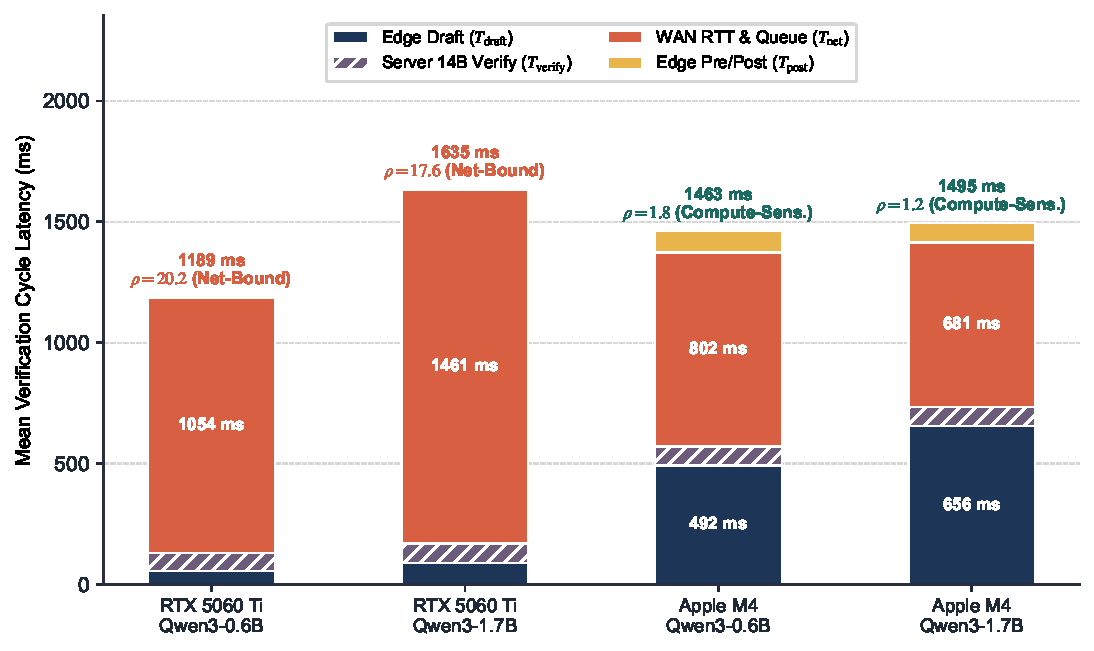
\includegraphics[width=\columnwidth]{figures_en/fig2_latency_breakdown.pdf}
  \caption{Exp.\ 2: Per-cycle latency breakdown and bottleneck ratio $\rho$ across the $2\times 2$ factorized matrix. RTX 5060 Ti spends over 92\% of cycle time waiting on WAN RTT ($\rho \in [17.65, 20.16]$), whereas Apple M4 splits cycle time nearly evenly between local drafting and WAN wait ($\rho \in [1.16, 1.79]$).}
  \label{fig:lat}
\end{figure}

\begin{figure*}[t]
  \centering
  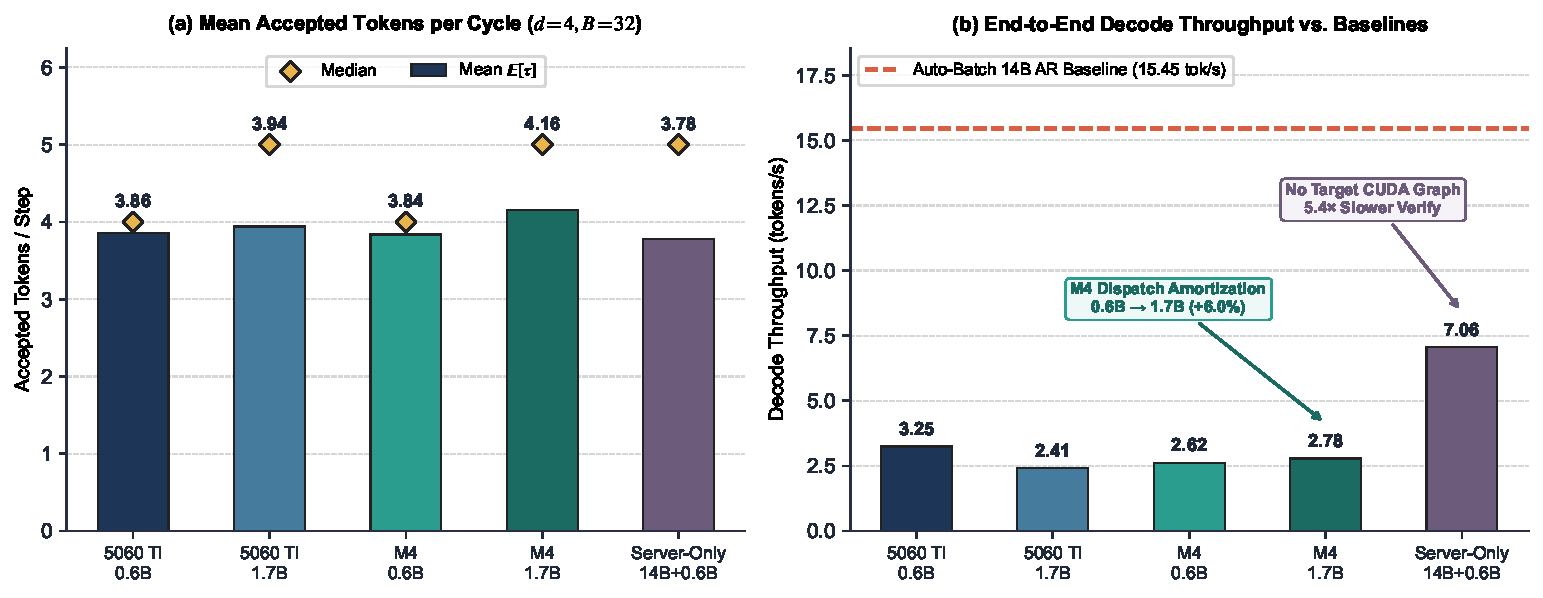
\includegraphics[width=0.95\textwidth]{figures_en/fig3_matrix_mat_throughput.pdf}
  \caption{Exp.\ 1 \& 2: Cross-impact of draft model scale and hardware backend on (a)~mean/median accepted tokens per cycle and (b)~end-to-end decode throughput relative to single-server baselines.}
  \label{fig:mat}
\end{figure*}

\textbf{1) Single-GPU VRAM Contention Proves the Value of Edge Offloading:} Even on a 32\,GB RTX 4080 SUPER, co-locating \texttt{Qwen3-14B} and \texttt{Qwen3-0.6B} (\texttt{E1-2}) leaves insufficient memory headroom to enable CUDA Graphs for the target model. As a result, single-step verification degrades to 431.6\,ms---$5.4\times$ slower than our dedicated edge-assisted server (75--82\,ms)---dropping \texttt{Server-Only} throughput to 7.06\,tok/s, well below pure autoregressive decoding (15.45\,tok/s). Offloading drafting to the edge frees server VRAM for full 14B CUDA Graph capture; projected to a sub-millisecond LAN ($T_{\mathrm{net}} < 1$\,ms), \texttt{5060 Ti + 1.7B} would deliver $3.94 / (0.0875 + 0.078) = 23.8$\,tok/s, a $1.54\times$ speedup over the 14B autoregressive baseline.

\textbf{2) Sharp Regime Bifurcation Between Edges:} At identical draft scales, RTX 5060 Ti's CUDA Graph engine drafts $7.5\times$--$8.8\times$ faster than Apple M4's eager MPS backend (56.0 vs.\ 492.4\,ms at 0.6B; 87.5 vs.\ 655.9\,ms at 1.7B) and performs client pre/post-processing $20\times$ faster (4.0 vs.\ 80--90\,ms). Yet over our Tailscale WAN, 5060 Ti experiences $\rho \in [17.65, 20.16]$ (over 92\% of cycle time spent in network wait), placing it deep in the \emph{network-bound} regime, whereas M4 exhibits $\rho \in [1.16, 1.79]$, placing it firmly in the \emph{compute-sensitive} regime.

\textbf{3) Fixed Dispatch-Overhead Amortization on Apple M4:} Scaling Apple M4's draft model nearly $3\times$ from \texttt{0.6B} (\texttt{E2-3}) to \texttt{1.7B} (\texttt{E2-4}) increases draft latency by only 33.2\% (492.4 $\to$ 655.9\,ms), while raising $\mathbb{E}[\tau]$ to the highest value in Exp.\ 2 (\textbf{4.16}, $+8.3\%$) and boosting end-to-end throughput by \textbf{+6.0\%} (2.62 $\to$ 2.78\,tok/s). This empirically confirms~(\ref{eq:amort}): PyTorch MPS incurs a $\sim 350$--400\,ms fixed host-dispatch floor per cycle, which larger draft models amortize effectively whenever unified memory permits.

\subsection{Proactive Drafting Ablation over WAN (Exp.\ 3)}

Table~\ref{tab:e3} and Fig.~\ref{fig:pro} evaluate all three Proactive Drafting strategies (\texttt{disabled}, \texttt{excluded}, \texttt{included}) under real WAN RTTs. Unlike LAN environments where short wait windows can starve proactive drafting, our 500--1500\,ms WAN wait windows give both edges ample idle time to complete next-cycle speculative trees before the server responds. Merging proactive candidates directly into the next tree (\texttt{included}) outperforms both alternatives across both architectures: on \texttt{5060 Ti (1.7B)}, \texttt{included} cuts mean draft latency by \textbf{-18.7\%} (88.9 $\to$ 72.3\,ms) and lifts throughput by \textbf{+17.0\%} over \texttt{disabled} (2.83 $\to$ 3.31\,tok/s); on \texttt{Apple M4 (0.6B)}, it compresses draft latency by \textbf{-14.6\%} (512.4 $\to$ 437.4\,ms) and achieves \textbf{3.47\,tok/s} (\textbf{+32.4\%} over default \texttt{excluded} and $+6.8\%$ over \texttt{disabled}).

\begin{table*}[t]
  \centering
  \caption{Exp.\ 3: Proactive Drafting Ablation across Heterogeneous WAN Edges ($d{=}4, B{=}32$)}
  \label{tab:e3}
  \begin{tabular}{llcccccc}
    \toprule
    Edge Link & Proactive Mode & $\mathbb{E}[\tau]$ & Proactive Hits / Steps & Draft (ms) & Wait (ms) & Throughput (tok/s) & Relative Gain \\
    \midrule
    \multirow{3}{*}{\texttt{5060 Ti (1.7B)}} & \texttt{disabled} & 3.60 & 0 / 254 & 88.9 & 1178.4 & 2.83 & Baseline \\
     & \texttt{excluded} (Default) & \textbf{3.94} & 36 / 236 & 87.5 & 1543.2 & 2.41 & WAN RTT spike \\
     & \textbf{\texttt{included} (Merged)} & 3.70 & \textbf{41 / 245} & \textbf{72.3 (-18.7\%)} & 1042.2 & \textbf{3.31} & \textbf{+17.0\%} \\
    \midrule
    \multirow{3}{*}{\texttt{Apple M4 (0.6B)}} & \texttt{disabled} & 3.71 & 0 / 242 & 512.4 & 497.8 & 3.25 & Baseline \\
     & \texttt{excluded} (Default) & \textbf{3.84} & 28 / 241 & 492.4 & 880.5 & 2.62 & WAN RTT spike \\
     & \textbf{\texttt{included} (Merged)} & 3.82 & \textbf{34 / 242} & \textbf{437.4 (-14.6\%)} & 583.4 & \textbf{3.47} & \textbf{+32.4\%*} \\
    \bottomrule
  \end{tabular}
  \\[2pt]\footnotesize * Gain relative to default \texttt{excluded} mode ($+6.8\%$ relative to \texttt{disabled}).
\end{table*}

\begin{figure*}[t]
  \centering
  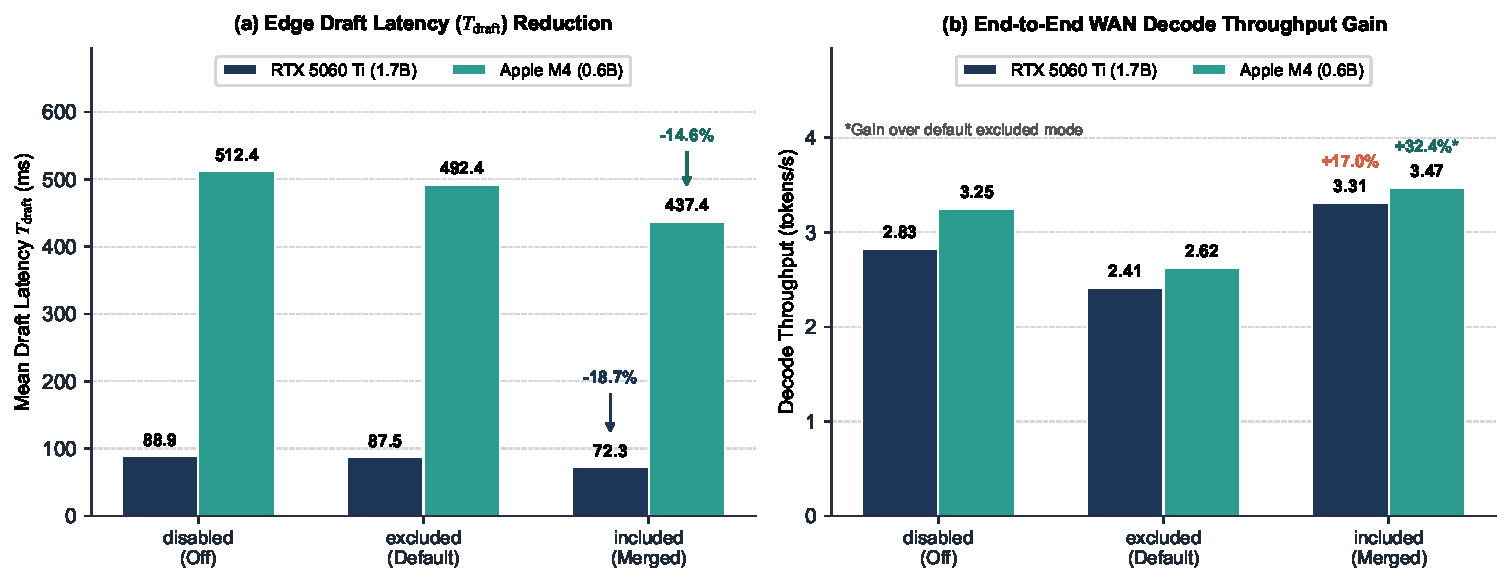
\includegraphics[width=0.95\textwidth]{figures_en/fig4_proactive_ablation.pdf}
  \caption{Exp.\ 3: Proactive Drafting ablation comparing \texttt{disabled}, \texttt{excluded}, and \texttt{included} modes on (a)~edge draft latency $T_{\mathrm{draft}}$ and (b)~end-to-end WAN decode throughput.}
  \label{fig:pro}
\end{figure*}

\subsection{Tree-Depth Sweep and Analytical Model Validation (Exp.\ 4a)}

Table~\ref{tab:e4a} and Fig.~\ref{fig:sweep} validate our closed-form model~(\ref{eq:tpot}) and Proposition~\ref{prop:bifurcation}. Linear regression of draft latency against depth $d$ confirms a \textbf{5.78$\times$} marginal cost gap: $\alpha_{\text{5060Ti}} = 22.4$\,ms/layer versus $\alpha_{\text{M4}} = 129.5$\,ms/layer. (Note that run \texttt{E4-1} at $(2,16)$ captured 5 requests / 85 decode steps due to a transient WAN drop, while all other runs completed all 16 prompts.) To remove stochastic WAN routing jitter when checking functional shape, Fig.~\ref{fig:sweep}(b) normalizes each edge to its typical reference waiting time (1150\,ms for 5060 Ti; 520\,ms for M4). The closed-form curves match the empirical points tightly ($R^2 = 0.992$ on 5060 Ti) and expose two opposite optima:
\begin{itemize}
  \item \textbf{RTX 5060 Ti (Monotonic Deep-Tree Gain):} Deepening the tree from $(2, 16)$ to $(8, 64)$ drives $\mathbb{E}[\tau]$ up from 2.88 to \textbf{5.84} (with peak single-step acceptance reaching \textbf{14 tokens}), reducing normalized TPOT by \textbf{-45\%} (413.2 $\to$ 226.9\,ms/tok).
  \item \textbf{Apple M4 (Shallow-Tree Optimum):} Shrinking the tree to $(2, 16)$ halves M4's local draft time (492.4 $\to$ \textbf{242.7\,ms}), reaching the highest single-client WAN throughput in our entire study (\textbf{3.55\,tok/s}, $+35.5\%$ over default $(4,32)$). Pushing M4 deeper to $d{=}4$ and $d{=}6$ inflates draft time to 760.7\,ms and causes normalized TPOT to rebound (261.5 $\to$ 263.8 $\to$ 272.2\,ms/tok).
\end{itemize}

\begin{table*}[t]
  \centering
  \caption{Exp.\ 4a: Speculation Tree Depth \& Budget Sweep and Normalized TPOT Verification}
  \label{tab:e4a}
  \begin{tabular}{lccccccc}
    \toprule
    Device \& Model & Tree $(d, B)$ & $\mathbb{E}[\tau]$ & Max Acc. & Draft (ms) & Per-Layer Slope $\alpha$ & Measured Tput & Norm.\ TPOT \\
    \midrule
    \multirow{4}{*}{\texttt{5060 Ti (1.7B)}} & $(2, 16)^{\dagger}$ & 2.88 & 5 & 41.1 & \multirow{4}{*}{22.4\,ms/layer} & 3.03\,tok/s & 413.2\,ms/tok \\
     & $(4, 32)$ & 3.94 & 8 & 87.5 & & 2.41\,tok/s & 314.0\,ms/tok \\
     & $(6, 48)$ & 4.80 & 8 & 132.4 & & 2.35\,tok/s & 267.1\,ms/tok \\
     & \textbf{$(8, 64)$} & \textbf{5.84} & \textbf{14} & 175.8 & & 2.90\,tok/s & \textbf{226.9 (-45\%)} \\
    \midrule
    \multirow{3}{*}{\texttt{Apple M4 (0.6B)}} & \textbf{$(2, 16)$} & 2.92 & 5 & \textbf{242.7} & \multirow{3}{*}{129.5\,ms/layer} & \textbf{3.55\,tok/s} & \textbf{261.5 (Opt.)} \\
     & $(4, 32)$ & 3.84 & 8 & 492.4 & & 2.62\,tok/s & 263.8\,ms/tok \\
     & $(6, 48)$ & 4.71 & 11 & 760.7 & & 2.95\,tok/s & 272.2 (Rebound) \\
    \bottomrule
  \end{tabular}
  \\[2pt]\footnotesize $^{\dagger}$ 5 requests (85 decode steps) collected prior to a transient Tailscale route reset; all other points span all 16 prompts.
\end{table*}

\begin{figure*}[t]
  \centering
  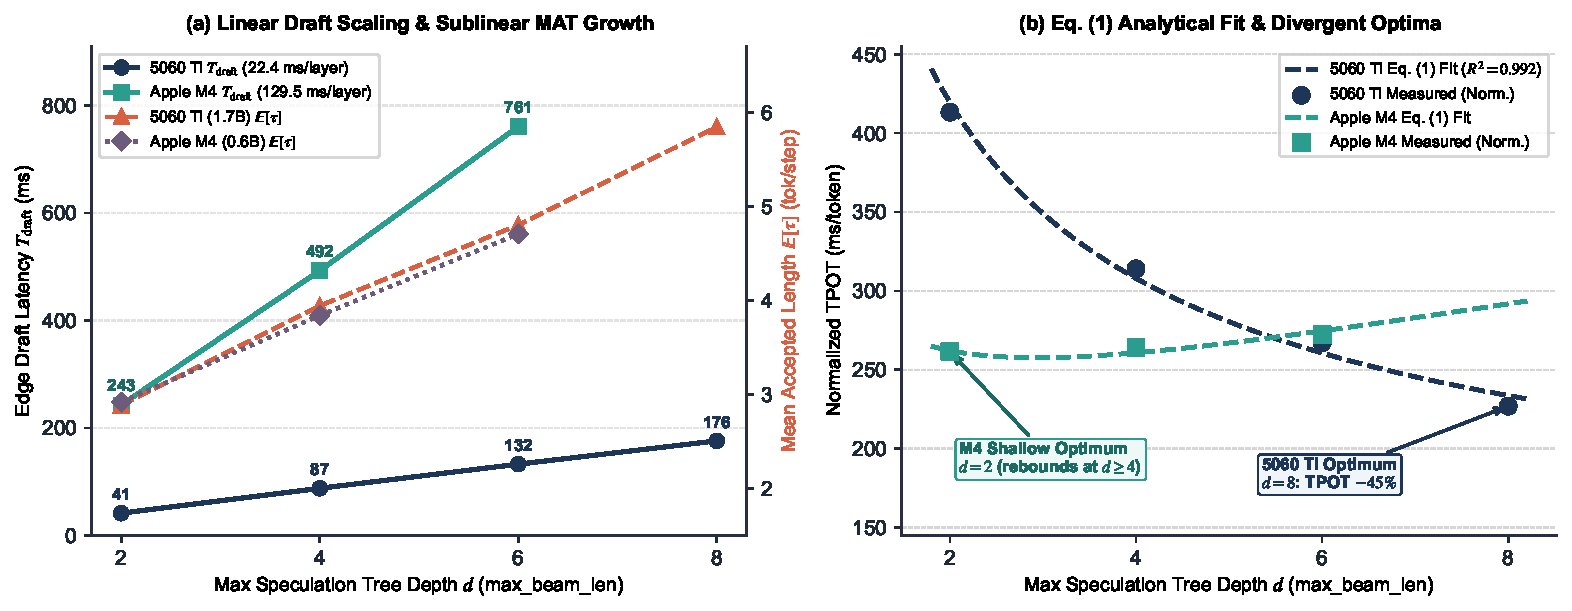
\includegraphics[width=0.95\textwidth]{figures_en/fig5_tree_sweep_theory_fit.pdf}
  \caption{Exp.\ 4a: (a)~Linear draft latency scaling ($5.78\times$ slope gap) and sublinear $\mathbb{E}[\tau]$ growth; (b)~Eq.~(\ref{eq:tpot}) closed-form model fit against reference-RTT-normalized measurements, confirming opposite optimal tree depths for RTX 5060 Ti ($d{=}8$) and Apple M4 ($d{=}2$).}
  \label{fig:sweep}
\end{figure*}

\subsection{Three-Node Concurrent End-to-End Evaluation (Exp.\ 4b)}

Finally, we evaluate Algorithm~\ref{alg:varbudget} under true simultaneous three-node concurrency (one 4080S server verifying both 5060 Ti and M4 concurrently across 16 prompts each). Table~\ref{tab:e4b} and Fig.~\ref{fig:e4b} contrast uniform default SpecEdge (\texttt{E4-Base}) against our heterogeneity-aware policy with Variable-Budget Zero-Padding (\texttt{E4-Opt}):
\begin{itemize}
  \item \textbf{Negligible Server Overhead:} Serving heterogeneous $B{=}64$ and $B{=}16$ trees from a single captured CUDA Graph increases median 14B server verification latency by only \textbf{+2.0\,ms} (76.0 $\to$ 78.0\,ms), confirming zero-padding adds virtually no runtime cost and zero extra VRAM.
  \item \textbf{Major Straggler Acceleration:} Reconfiguring the network-bound 5060 Ti edge to $(d{=}8, B{=}64, \texttt{included})$ raises its $\mathbb{E}[\tau]$ by \textbf{+41.3\%} (3.90 $\to$ 5.51), eliminates \textbf{28.9\%} of WAN verification RPCs (235 $\to$ 167), lowers TPOT by \textbf{-36.6\%} (631.7 $\to$ 400.6\,ms), and increases decode throughput by \textbf{+57.7\%} (1.58 $\to$ 2.50\,tok/s).
  \item \textbf{Massive Laptop Compute Savings \& Cluster Fairness:} Switching Apple M4 to $(d{=}2, B{=}16, \texttt{included})$ slashes local GPU draft latency by \textbf{-64.0\%} (481.7 $\to$ 173.5\,ms, with 104/334 proactive hits = 31.1\%)---directly curbing thermal throttling and battery drain on thin-and-light laptops. Although M4's raw throughput dipped modestly (-12.1\% due to a +72\,ms concurrent WAN wait fluctuation), cluster aggregate throughput rose by \textbf{+9.7\%} (5.06 $\to$ 5.56\,tok/s), and the max/min inter-edge throughput imbalance dropped by \textbf{44.1\%} (from $2.20\times$ to $1.23\times$).
\end{itemize}

\begin{table}[t]
  \centering
  \caption{Exp.\ 4b: Three-Node Concurrent Comparison (\texttt{E4-Base} vs.\ \texttt{E4-Opt})}
  \label{tab:e4b}
  \setlength{\tabcolsep}{3.6pt}
  \begin{tabular}{lccc}
    \toprule
    Metric & \texttt{E4-Base} & \texttt{E4-Opt} & Delta \\
    \midrule
    5060 Ti $\mathbb{E}[\tau]$ / RPCs & 3.90 / 235 & \textbf{5.51 / 167} & \textbf{+41.3\% / -28.9\%} \\
    5060 Ti TPOT & 631.7\,ms & \textbf{400.6\,ms} & \textbf{-36.6\%} \\
    5060 Ti Throughput & 1.58\,tok/s & \textbf{2.50\,tok/s} & \textbf{+57.7\%} \\
    M4 Draft Latency & 481.7\,ms & \textbf{173.5\,ms} & \textbf{-64.0\%} \\
    M4 Throughput & 3.48\,tok/s & 3.06\,tok/s & -12.1\% \\
    Server 14B Verify & 76.0\,ms & \textbf{78.0\,ms} & +2.0\,ms \\
    \midrule
    \textbf{Aggregate Tput} & 5.06\,tok/s & \textbf{5.56\,tok/s} & \textbf{+9.7\%} \\
    \textbf{Imbalance (Max/Min)} & $2.20\times$ & \textbf{$1.23\times$} & \textbf{-44.1\%} \\
    \bottomrule
  \end{tabular}
\end{table}

\begin{figure*}[t]
  \centering
  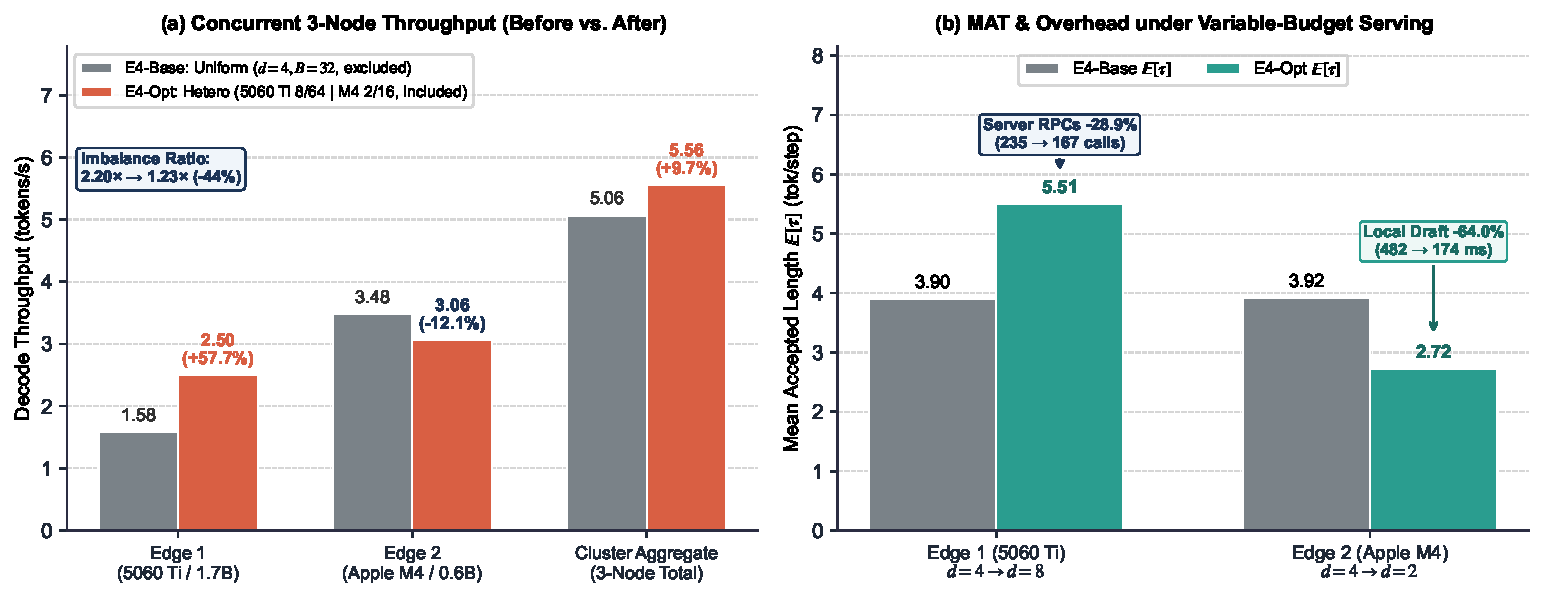
\includegraphics[width=0.95\textwidth]{figures_en/fig6_3node_before_after.pdf}
  \caption{Exp.\ 4b: Concurrent three-node evaluation comparing uniform default SpecEdge (\texttt{E4-Base}) against heterogeneity-aware Variable-Budget serving (\texttt{E4-Opt}). (a)~Per-edge and aggregate throughput with imbalance ratio reduction; (b)~$\mathbb{E}[\tau]$ shift, RPC reduction, and local draft latency savings.}
  \label{fig:e4b}
\end{figure*}

\section{Deployment Guidelines, Limitations, and Future Work}

\subsection{Actionable Guidelines for Heterogeneous Edge-Cloud Serving}

Our theoretical model and empirical findings distill into three deployment rules for practitioners building commodity device-cloud LLM clusters:
\begin{enumerate}
  \item \textbf{Partition Policies by Bottleneck Ratio $\rho$:} Measure baseline $T_{\mathrm{draft}}$ and $T_{\mathrm{wait}}$ over a short warm-up window. Assign deep trees ($d{=}6$--$8, B{=}48$--$64$) with \texttt{proactive=included} whenever $\rho > 5$, and shallow trees ($d{=}2$--$3, B{=}16$--$24$) with \texttt{included} whenever $\rho \le 2$.
  \item \textbf{Match Draft Capacity to Dispatch Floor:} On eager backends with high fixed launch overhead (such as PyTorch MPS), prefer mid-sized draft models (e.g., 1.7B over 0.6B) whenever unified memory allows, leveraging higher acceptance to amortize dispatch costs.
  \item \textbf{Server Storage and Memory Hygiene:} When serving multi-tens-of-GB target models inside WSL2, always stage checkpoints on native \texttt{ext4} volumes rather than cross-OS 9p mounts, and reserve headroom for a single maximum-budget CUDA Graph via zero-padding rather than capturing multiple graph buckets.
\end{enumerate}

\subsection{Limitations and Future Directions}

First, while our compatibility layer enables seamless Apple Silicon execution via PyTorch MPS, eager dispatch still imposes $\sim 129.5$\,ms/layer on M4; replacing the client draft engine with Apple's native Metal graph-compiled \textbf{MLX} framework while retaining our gRPC protocol could potentially narrow the draft-latency gap to $\sim 50$\,ms. Second, real WAN links exhibit second-scale RTT jitter. Because our Variable-Budget Zero-Padding server already accepts arbitrary $K \le B_{\max}+1$ per request without restarting or recompiling, a natural next step is an \emph{online sliding-window RTT controller} on each edge client that dynamically adjusts $(d_t, B_t)$ step-by-step according to instantaneous $\hat{\rho}_t$.

\section{Conclusion}

We presented an analytical, architectural, and empirical study of edge-cloud speculative decoding on heterogeneous cross-platform wide-area clusters. Starting from a counter-intuitive throughput inversion observed between an RTX 5060 Ti desktop GPU and an Apple M4 laptop, we derived a cycle-level TPOT model and dimensionless bottleneck ratio $\rho$ that accurately explains divergent optimal tree depths ($R^2{=}0.992$) as well as eager dispatch-overhead amortization. On the systems side, we built a non-intrusive Apple MPS compatibility layer and proposed Variable-Budget Static CUDA Graph Zero-Padding, enabling a single 14B target graph to serve heterogeneous tree budgets with exact mathematical equivalence and only $+2.0$\,ms overhead. Real three-node concurrent experiments confirm $+57.7\%$ bottleneck speedup, $-64.0\%$ laptop draft compute savings, $+9.7\%$ aggregate cluster throughput gain, and a $44.1\%$ reduction in inter-edge imbalance, providing a practical foundation for real-world heterogeneous device-cloud LLM serving.

\begin{thebibliography}{12}
\bibitem{leviathan2023spec}
Y.~Leviathan, M.~Kalman, and Y.~Matias, ``Fast inference from transformers via speculative decoding,'' in \emph{Proc. 40th Int. Conf. Mach. Learn. (ICML)}, 2023, pp.~19274--19286.

\bibitem{chen2023accelerating}
C.~Chen, S.~Borgeaud, G.~Irving, J.-B.~Lespiau, L.~Sifre, and J.~Jumper, ``Accelerating large language model decoding with speculative sampling,'' \emph{arXiv preprint arXiv:2302.01318}, 2023.

\bibitem{cai2024medusa}
T.~Cai, Y.~Li, Z.~Geng, H.~Peng, J.~D.~Lee, D.~Chen, and T.~Dao, ``Medusa: Simple LLM inference acceleration framework with multiple decoding heads,'' in \emph{Proc. 41st Int. Conf. Mach. Learn. (ICML)}, 2024.

\bibitem{li2024eagle}
Y.~Li, F.~Wei, C.~Zhang, and H.~Zhang, ``EAGLE: Speculative sampling requires rethinking feature uncertainty,'' in \emph{Proc. 41st Int. Conf. Mach. Learn. (ICML)}, 2024.

\bibitem{svirschevski2024specexec}
R.~Svirschevski, A.~May, Z.~Chen, B.~Chen, Z.~Jia, and M.~Ryabinin, ``SpecExec: Massively parallel speculative decoding for interactive LLM inference on consumer devices,'' in \emph{Advances in Neural Information Processing Systems (NeurIPS)}, 2024.

\bibitem{kang2017neurosurgeon}
Y.~Kang, J.~Hauswald, C.~Gao, A.~Rovinski, T.~Mudge, J.~Mars, and L.~Tang, ``Neurosurgeon: Collaborative intelligence between the cloud and mobile edge,'' in \emph{Proc. 22nd Int. Conf. Architectural Support for Programming Languages and Operating Systems (ASPLOS)}, 2017, pp.~615--629.

\bibitem{hao2024hybrid}
Z.~Hao, H.~Jiang, S.~Jiang, J.~Ren, and T.~Cao, ``Hybrid SLM and LLM for edge-cloud collaborative inference,'' in \emph{Proc. Workshop on Edge and Mobile Foundation Models (EdgeFM)}, 2024.

\bibitem{park2025specedge}
J.~Park, S.~Cho, and D.~Han, ``SpecEdge: Scalable edge-assisted serving framework for interactive LLMs,'' in \emph{Advances in Neural Information Processing Systems (NeurIPS)}, 2025, arXiv:2505.17052.

\bibitem{kwon2023vllm}
W.~Kwon, Z.~Li, S.~Zhuang, Y.~Sheng, L.~Zheng, C.~H.~Yu, J.~Gonzalez, H.~Zhang, and I.~Stoica, ``Efficient memory management for large language model serving with PagedAttention,'' in \emph{Proc. 29th Symp. Operating Systems Principles (SOSP)}, 2023, pp.~611--626.

\bibitem{qwen3}
Qwen Team, ``Qwen3 technical report,'' Alibaba Cloud, Tech.\ Rep., 2025.

\bibitem{liu2024specbench}
X.~Liu, L.~Hu, P.~Bailis, I.~Stoica, Z.~Deng, A.~Cheung, and H.~Zhang, ``SpecBench: A comprehensive benchmark for speculative decoding,'' \emph{arXiv preprint arXiv:2401.07851}, 2024.

\bibitem{agrawal2024sarathi}
A.~Agrawal, N.~Kedia, A.~Panwar, J.~Mohan, N.~Kwatra, B.~S.~Gulavani, A.~Tumanov, and R.~Ramjee, ``Taming throughput-latency tradeoff in LLM inference with Sarathi-Serve,'' in \emph{Proc. 18th USENIX Symp. Operating Systems Design and Implementation (OSDI)}, 2024, pp.~117--134.
\end{thebibliography}

\end{document}
